\documentclass{beamer}
\mode<presentation>
\usepackage{amsmath,amssymb,mathtools}
\usepackage{textcomp}
\usepackage{gensymb}
\usepackage{adjustbox}
\usepackage{subcaption}
\usepackage{enumitem}
\usepackage{multicol}
\usepackage{listings}
\usepackage{url}
\usepackage{graphicx} % <-- needed for images
\def\UrlBreaks{\do\/\do-}

\usetheme{Boadilla}
\usecolortheme{lily}
\setbeamertemplate{footline}{
  \leavevmode%
  \hbox{%
  \begin{beamercolorbox}[wd=\paperwidth,ht=2ex,dp=1ex,right]{author in head/foot}%
    \insertframenumber{} / \inserttotalframenumber\hspace*{2ex}
  \end{beamercolorbox}}%
  \vskip0pt%
}
\setbeamertemplate{navigation symbols}{}

\lstset{
  frame=single,
  breaklines=true,
  columns=fullflexible,
  basicstyle=\ttfamily\tiny   % tiny font so code fits
}

\numberwithin{equation}{section}

% ---- your macros ----
\providecommand{\nCr}[2]{\,^{#1}C_{#2}}
\providecommand{\nPr}[2]{\,^{#1}P_{#2}}
\providecommand{\mbf}{\mathbf}
\providecommand{\pr}[1]{\ensuremath{\Pr\left(#1\right)}}
\providecommand{\qfunc}[1]{\ensuremath{Q\left(#1\right)}}
\providecommand{\sbrak}[1]{\ensuremath{{}\left[#1\right]}}
\providecommand{\lsbrak}[1]{\ensuremath{{}\left[#1\right.}}
\providecommand{\rsbrak}[1]{\ensuremath{\left.#1\right]}}
\providecommand{\brak}[1]{\ensuremath{\left(#1\right)}}
\providecommand{\lbrak}[1]{\ensuremath{\left(#1\right.}}
\providecommand{\rbrak}[1]{\ensuremath{\left.#1\right)}}
\providecommand{\cbrak}[1]{\ensuremath{\left\{#1\right\}}}
\providecommand{\lcbrak}[1]{\ensuremath{\left\{#1\right.}}
\providecommand{\rcbrak}[1]{\ensuremath{\left.#1\right\}}}
\theoremstyle{remark}
\newtheorem{rem}{Remark}
\newcommand{\sgn}{\mathop{\mathrm{sgn}}}
\providecommand{\abs}[1]{\left\vert#1\right\vert}
\providecommand{\res}[1]{\Res\displaylimits_{#1}}
\providecommand{\norm}[1]{\lVert#1\rVert}
\providecommand{\mtx}[1]{\mathbf{#1}}
\providecommand{\mean}[1]{E\left[ #1 \right]}
\providecommand{\fourier}{\overset{\mathcal{F}}{ \rightleftharpoons}}
\providecommand{\system}{\overset{\mathcal{H}}{ \longleftrightarrow}}
\providecommand{\dec}[2]{\ensuremath{\overset{#1}{\underset{#2}{\gtrless}}}}
\newcommand{\myvec}[1]{\ensuremath{\begin{pmatrix}#1\end{pmatrix}}}
\let\vec\mathbf

\title{MatGeo Presentation - Problem 9.2.32}
\author{EE25BTECH11064 - Yojit Manral}
\date{}

\begin{document}

\frame{\titlepage}
\begin{frame}{Question}
Find the area of the region included between $y^2 = 9x$ and $y = x$.
\end{frame}

\begin{frame}{Solution}
$\rightarrow$ The given conic can be expressed with parameters
\begin{align}
    \vec{V} = \myvec{0&0\\0&1}\text{, } \vec{u} = \myvec{-\frac{9}{2}\\0}\text{, } f = 0
\end{align}
$\rightarrow$ The given line can be expressed with the parameters
\begin{align}
    \vec{h} = \myvec{0\\0}\text{, } \vec{m} = \myvec{1\\1}
\end{align}
$\rightarrow$ The point of intersection of the line
\begin{align}
    \vec{L} \equiv \vec{x} = \vec{h} + \kappa\vec{m}
\end{align}
\hspace{0.3cm} with a general conic
\begin{align}
    g\brak{\vec{x}} = \vec{x}^T\vec{V}\vec{x} + 2\vec{u}^T\vec{x} + f = 0
\end{align}
\hspace{0.3cm} can be given by
\begin{align}
    \vec{x_i} = \vec{h} + \kappa_i\vec{m}
\end{align}
\end{frame}

\begin{frame}{Solution}
\hspace{0.3cm} where
\begin{align}
    \kappa_i = \frac{1}{\vec{m}^T\vec{V}\vec{m}}\brak{-\vec{m}^T\brak{\vec{V}\vec{h}+\vec{u}}\pm \sqrt{\brak{\vec{m}^T\brak{\vec{V}\vec{h}+\vec{u}}}^2-g\brak{\vec{h}}\brak{\vec{m}^T\vec{V}\vec{m}}}}
\end{align}
$\rightarrow$ Substituting the parameters from (1), (2) in (6), we get
\begin{align}
    \vec{x_1} = \myvec{0\\0}\text{, } \vec{x_2} = \myvec{9\\9}
\end{align}
$\rightarrow$ From the figure, the area bounded by the conic $y^2 = 9x$ and the line $y = x$ is given by
\begin{align}
    \int_{0}^{9}\brak{3\sqrt{x} - x}dx &= \left[2(x)^{3/2} - \frac{x^2}{2}\right]_{0}^{9} \\
    &= \frac{27}{2}\hspace{0.2cm}units
\end{align}
\end{frame}

\begin{frame}{Solution}
\begin{figure}[h!]
   \centering
   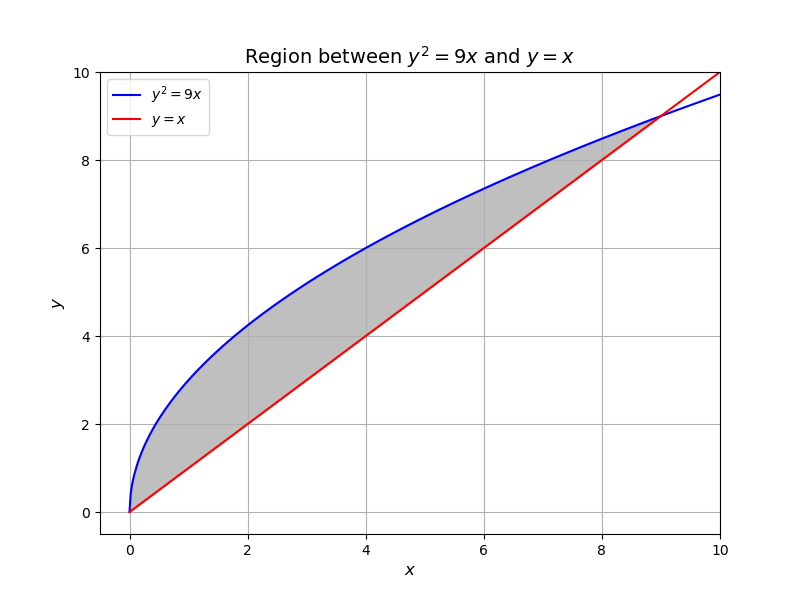
\includegraphics[width=0.85\linewidth]{figs/01.png}
   \caption{Plot of $y^2 = 9x$ and $y = x$}
   \label{Plot_1}
\end{figure}
\end{frame}
 % --------- CODE APPENDIX ---------
% Python plotting
\begin{frame}[fragile]{File: plot.py}
\begin{lstlisting}[language=Python]
import numpy as np
import matplotlib.pyplot as plt

# Define the functions
def curve1(x):
    return np.sqrt(9 * x)

def curve2(x):
    return x

# Define the x-range
x = np.linspace(0, 10, 500)

# Plot the curves
plt.figure(figsize=(8, 6))
plt.plot(x, curve1(x), label=r"$y^2 = 9x$", color="blue")
plt.plot(x, curve2(x), label=r"$y = x$", color="red")

# Fill the region between the curves
plt.fill_between(x, curve2(x), curve1(x), where=(curve2(x) <= curve1(x)), color="gray", alpha=0.5)

# Add labels and title
plt.title("Region between $y^2 = 9x$ and $y = x$", fontsize=14)
plt.xlabel("$x$", fontsize=12)
plt.ylabel("$y$", fontsize=12)
plt.legend()

# Show the plot
plt.grid(True)
plt.xlim(-0.5, 10)
plt.ylim(-0.5, 10)
plt.show()
\end{lstlisting}
\end{frame}

\end{document}
